\setchapterpreamble[u]{\margintoc}
\chapter{Fusion of UAS-based image datasets}
\labch{image_fusion}
\label{sec:image_fusion}

\section*{About this chapter}

This chapter describes the image registration algorithm on which this dissertation is articulated. The matching of multispectral and thermographic images with visible information is here addressed. To this end, the Enhanced Correlation Coefficient (\acrshort{ecc}) is used for maximizing the correlation of images in different spectral ranges. A comparative assessment is finally done to demonstrate which is the best configuration to balance both time efficiency and quality of matching results. Shortcomings that are frequent in remotely sensed aerial images were presented and solved in Chapter \nameref{sec:materials}. 

\section{Matching multispectral imagery}

\begin{figure*}
    \includegraphics[width=\linewidth]{figs/image_fusion/summary_image_fusion.png}\hspace*{\fill}
    \caption{Fusion of multispectral, thermographic and RGB imagery compose a multi-layer model which is later applied on the characterization of individual trees.}
	\label{fig:image_fusion_framework}
\end{figure*}

The Parrot Sequoia multispectral sensor captures four spectral bands: Green (GRE), Red (RED), Red Edge (\acrshort{reg}) and Near Infrared (\acrshort{nir}). These are acquired by the same device but with different lenses aimed at perceiving different spectral wavelengths. If the images are overlapped as collected there is a lack of alignment among them, as exposed in Figure \ref{fig:multispectral_ghost_effect}. At least the following differences were identified: 
\begin{itemize}
    \item Images are translated as a result of each lens working in a \textbf{different fixed position within the multispectral sensor}. 
    \item \textbf{Every lens has its own optical axis and principal point}. The ideal configuration consists of parallel optical axes that help to solve the misalignment with a simple translation. Even if this was the configuration after manufacturing, the lens calibration deteriorates over time. Indeed, the image metadata shows the viewing conditions of each band with respect to the master one, Green, in what is known as a camera ring. It is defined as a set of cameras which are connected and defined by geometric constraints. Every band defines its own yaw, roll and pitch angles with respect to the master, and thus optical axes cannot be assumed to be parallel.
    \item \textbf{Timestamps differ for multispectral images belonging to the same shot}. It is in the order of \si{\milli\second}, and yet it implies a harder matching because of the \acrshort{uas}'s movement.
\end{itemize}

\begin{marginfigure}[.2cm]
  \includegraphics{figs/image_fusion/multispectral_ghost_effect.png}
  \caption{Image ghosting effect obtained by overlapping multispectral bands with $\alpha < 1$.}
  \label{fig:multispectral_ghost_effect}
\end{marginfigure}
Matching of multispectral imagery can be performed by means of the image metadata, thus relying on the sensor calibration. However, another approach is to match images using only colourimetric information. Traditional image-matching approaches, such as \acrshort{sift}, \acrshort{surf} and \acrshort{orb}, do not work well over images collecting different wavelength intervals, with surfaces showing different radiation. Although there exist variants from \acrshort{sift} that work under photometric differences \cite{park_pi-sift_2008}, they are not as robust as the \textbf{Enhanced Correlation Coefficient (\acrshort{ecc})} \cite{evangelidis_parametric_2008}. Given two images of the same dimensionality, \acrshort{ecc} seeks the matrix that minimizes the intensity correlation of both images. It is more convenient for our purposes for the following reasons. First, it works by estimating a transformation matrix, ranging from a simple translation ($2 \times 3$) to a homography ($3 \times 4$); the larger the matrix, the more time-consuming the process. Therefore, the motion model can be determined considering the desired time efficiency and what kind of transformations the misalignment presents. Even for the homography, the algorithm has a linear complexity ($\mathcal{O}(n)$). Control parameters of \acrshort{ecc} are the number of maximum iterations upon convergence ($n$) as well as the aimed precision ($\epsilon$). Another intrinsic parameter is the dimensionality of input images, as it considerably reduces latency.

\begin{marginfigure}[-2cm]
    \centering
    \includegraphics{figs/image_fusion/motion_models.png}
    \caption{Transformation models that can be estimated using \acrshort{ecc}.}
    \label{fig:ecc_motion_models}
\end{marginfigure}

\begin{figure}[ht]
    \centering
    \includegraphics[width=\linewidth]{figs/image_fusion/ecc_hierarchy.png}
    \caption{Hierarchical registration of multispectral imagery.}
	\label{fig:ecc_hierarchy}
\end{figure}

Homography can describe any kind of differences among images, but the Euclidean model was proven enough for matching multispectral bands. Hence, the algorithmic complexity was reduced by estimating a matrix of size $2 \times 3$, which can explain translation, rotation and scaling, with the first being the most relevant. The procedure can be further improved by first matching those images which are more similar in terms of intensity. According to the peculiarities of multispectral images, these are fused hierarchically rather than sequentially. With this approach, images with more similar intensity are first registered. More specifically, the next pipeline is followed: $\textit{GRE} \rightarrow \textit{RGB}$, $\textit{RED} \rightarrow \textit{GRE} \rightarrow \textit{RGB}$, $\textit{REG} \rightarrow \textit{GRE} \rightarrow \textit{RGB}$ and $\textit{NIR} \rightarrow \textit{REG} \rightarrow \textit{GRE} \rightarrow \textit{RGB}$ (see Figure \ref{fig:ecc_hierarchy}). Still, each image is only registered once, as the whole chain concatenation is computed using matrix composition. Though desirable, convergence is not always achieved by the algorithm for every pair of images. This scenario is identified by calculating the angles of the resulting quadrilateral shape. If an angle exceeds a threshold, $\beta$, the matching result is discarded to avoid highly distorted shapes. The transformed results may also have areas with undetermined values. Once again, the minimum area to be cropped can be calculated as defined in Equation \ref{eq:matrix_corners}. It cannot be simply computed from the lower left and upper right corners, $[0, 0]$ and $[w - 1, h - 1]$, since Euclidean transformations also involve rotations. Thus, it is not enough to check two non-adjacent corners.

The hierarchical alignment of multispectral images is constructed on the basis of the image similarity of multispectral bands, as shown in Figure \ref{fig:multi_band_correlation}. It shows the correlation between pairs of bands through the normalized correlation coefficient (\acrshort{cc}), which calculates a value $\rho \in [0,1]$ that show how similar two grayscale images are, $f(x, y)$, $f'(x, y)$. For the sake of simplicity, the Green image is considered the root as in the camera ring. Accordingly, Figure \ref{fig:multi_band_correlation} justifies the hierarchy shown in Figure \ref{fig:ecc_hierarchy}. Note that \acrshort{nir} and \acrshort{reg} layers are reciprocally the most similar. However, \acrshort{reg} images are more similar to the root, Green, and thus \acrshort{nir} layers were aligned to \acrfull{reg} images.

\begin{figure*}
    \centering
    \includegraphics{figs/image_fusion/confusion_matrices.png}
    \caption{Confusion matrices depicting the similarity of multispectral images in three different datasets.}
    \label{fig:multi_band_correlation}
\end{figure*}

\section{Matching \acrshort{rgb} and multispectral imagery}

\begin{figure*}
    \centering
    \includegraphics{figs/image_fusion/multispectral_rgb_registration.png}
    \caption{Image-matching for \acrshort{rgb} and multispectral datasets. The blur size was increased for a better understanding of the figure.}
    \label{fig:rgb_multi_registration}
\end{figure*}

The contribution of \acrshort{rgb} imagery to this model is to add more accurate geopositioning data. However, multispectral and \acrshort{rgb} datasets were not acquired by the same device in this work, nor they were synchronized on the triggering. Thus, images to be matched are selected according to the timestamp, and yet, their timestamp difference may scale up to several seconds. Similarly to the previous case study, the \acrshort{ecc} is appropriate since \acrshort{rgb} and multispectral images have some relevant differences in the depicted object intensity. Instead of matching every multispectral image, only the root was registered and therefore the rest is also matched according to the hierarchy proposed in Figure \ref{fig:ecc_hierarchy}.

\acrshort{rgb} images have higher dimensionality than multispectral images, and thus the former was downscaled to match the size of the latter. The \acrshort{ecc} algorithm can be applied at a sub-pixel level and its parameters can be configured for a fine-grained registration. Furthermore, faster convergence is achieved by blurring both images, despite being slower. The complete workflow is shown in Figure \ref{fig:thermal_registration}, whereas the values of the parameters are the following: a blur mask of size 3, a high number of iterations, $n \gets 400$, and a high precision factor, $p \gets 1^{-60}$. The values of these parameters are further discussed in Section \nameref{sec:image_fusion_evaluation}. Figure \ref{fig:rgb_multi_registration_result} shows an example of this matching procedure.

\begin{figure}[ht]
    \centering
    \includegraphics{figs/image_fusion/rgb_multispectral_registration_result.png}
    \caption{An example of image-matching between a multispectral and \acrshort{rgb} image. The original images are depicted on the right side.}
    \label{fig:rgb_multi_registration_result}
\end{figure}

\section{Matching \acrshort{rgb} and thermographic images}

\begin{figure*}
    \includegraphics{figs/image_fusion/thermal_registration.png}
    \caption{Flow chart of the image-matching procedure between \acrshort{rgb} and infrared imagery.}
    \label{fig:thermal_registration}
\end{figure*}

The last step of this multi-layer architecture is to match thermal and \acrshort{rgb} imagery, with \acrshort{rgb} images being the link among multispectral and thermal datasets. Shortcomings concerning capture asynchronism are here mitigated since both kinds of images are taken by the same device. Still, there exist huge differences in the optical acquisition of \acrshort{rgb} and thermal images. The \acrshort{rgb} lens captures a wider area following the fisheye distortion model, whereas the thermal lens has a more narrowed field of view. As occurred for multispectral images, there is a translation between both images due to the physical distance between lenses, as well as rotations derived from differences in the shot triggering despite being synchronized. Also, the parameters from the optical systems are not enough to determine which is the overlapping area of interest in both \acrshort{rgb} and thermal datasets. 

In this case study, the affine transformation of the \acrshort{ecc} model was selected as the optimizing objective. Translation and rotation help on addressing the visual differences in \acrshort{rgb} and thermal imagery, whereas scaling searches for an appropriate size where both images overlap and fit well. At least two approaches can be followed to solve their matching: a) select a bigger area of the \acrshort{rgb} image which entirely covers the thermal image, with the result including some null values, or b) select a smaller area which does not necessarily cover the thermal image, thus tackling the previous shortcoming (Figure \ref{fig:thermal_comparative}). The complete procedure is shown in Figure \ref{fig:thermal_registration}. \acrshort{rgb} images were downscaled to fit the thermal dimensionality and thus the response time is lowered. The precision factor and the number of iterations were adjusted to provide an accurate registration. 

\begin{figure}
    \includegraphics{figs/image_fusion/thermal_comparative.png}
    \caption{Matching of \acrshort{rgb} and thermal images using an \acrshort{rgb} area smaller than thermal images, whereas the result on the right side was obtained with a larger \acrshort{rgb} area. }
    \label{fig:thermal_comparative}
\end{figure}

\section{Segmentation of individual trees}

\begin{figure*}
	\centering
	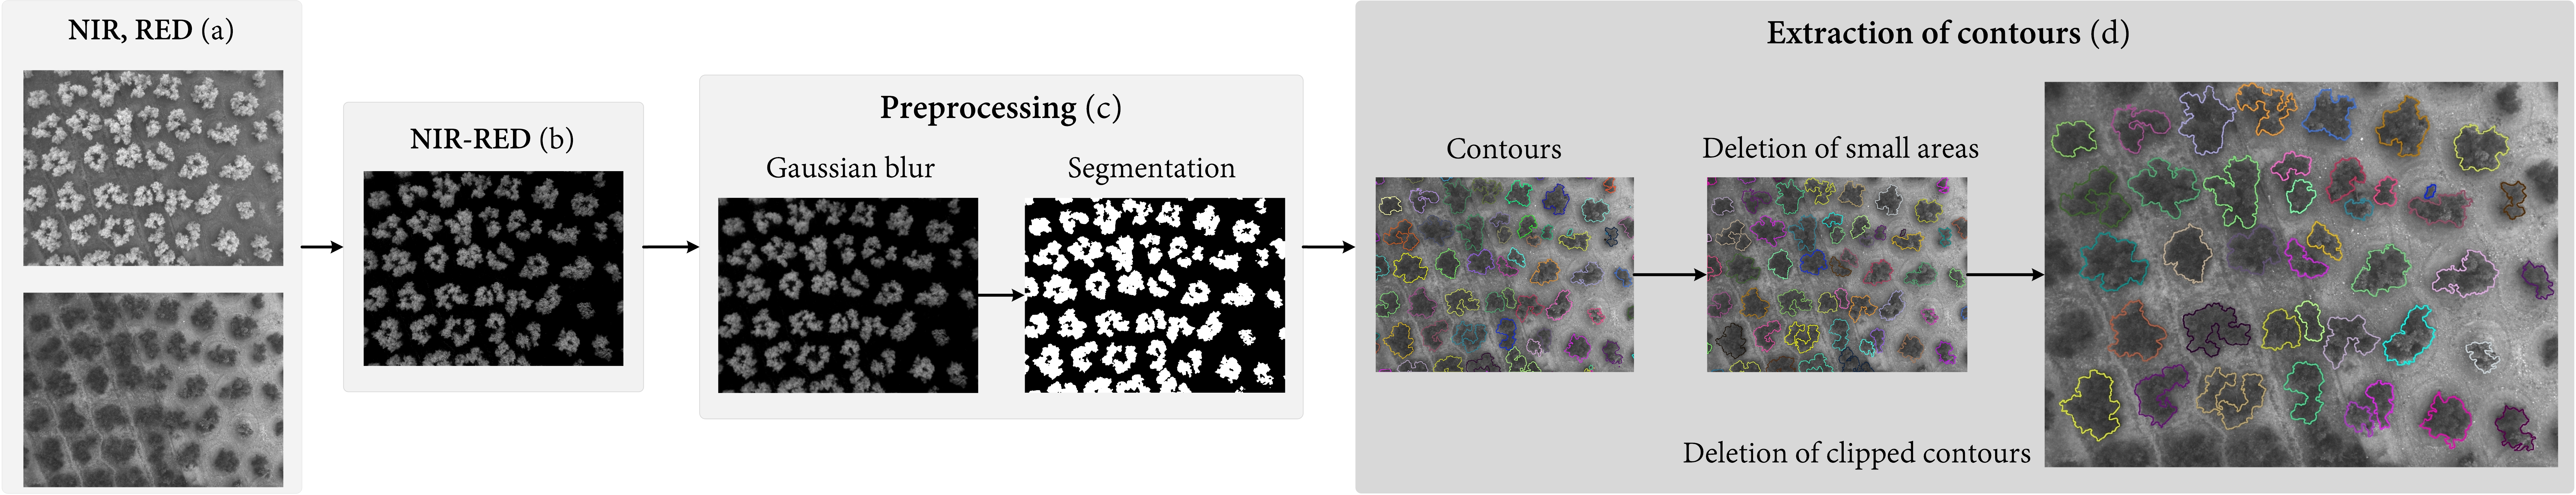
\includegraphics{figs/image_fusion/contour_retrieval.png}
	\caption{Transformation of multispectral images to distinguish vegetation and soil.}
	\label{fig:contour_extraction}
\end{figure*}

The proposed framework enables obtaining \acrshort{rgb}, multispectral and thermographic data from an area of interest. This stack of layers can be further applied to the temporal tracking of individual trees. More specifically, multispectral images are sensitive to vegetation and thus can help in the identification of trees. Once identified, points belonging to each one can be further analyzed to extract vegetation indices such as \acrshort{ndvi}. 

The observed surface reflectance, $f(\theta)$, presents some peaks where the vegetation reflectance reaches a maximum value. The contrast among layers with higher and lower reflectance enables distinguishing soil and canopy. Despite not having more fine-grained samples of $f(\theta)$ as in hyperspectral data, relative maximum and minimum reflectance values concerning vegetation are visible at \acrshort{nir} and Red layers, respectively. Soil reflectance is assumed to be constant or small throughout all these layers, and thus can be easily filtered out. Therefore, $\textit{\acrshort{nir}} - \textit{Red}$ produces the result shown in Figure \ref{fig:contour_extraction}.

Besides the image subtraction, the following steps are previously performed:
\begin{enumerate}
    \item \textbf{Gaussian blur} to smooth the image colour and remove noise.
    \item \textbf{Image thresholding} to isolate the vegetation-labelled pixels.
    \item \textbf{Extraction of the hierarchy of contours}. Contours inside another one are not of interest and therefore are discarded. Similarly, small contours belonging to low vegetation or noise
    as well as cropped contours (partially visible) are also discarded. The latter scenario can be identified since cropped shapes have horizontal or vertical edges on the image boundaries.
\end{enumerate}

The identification of individual trees is controlled using the size of a blur mask, the maximum area to be discarded and a threshold value, which must be high enough to avoid merging close trees. Although this procedure estimates shapes with high \acrshort{lod}, most of them have hundreds of points that can be narrowed down with a convex hull \cite{sklansky_finding_1982} or other polygons (e.g., hexagons). 

\begin{figure}[hbp]
    \centering
    \includegraphics[width=1\linewidth]{figs/image_fusion/convex_hull_contours.png}
    \caption{Conversion of polygons into convex and hexagonal hulls.}
    \label{fig:convex_hull_contours}
\end{figure}

\section{Results and discussion}
\label{sec:image_fusion_evaluation}

This work has been evaluated with four different datasets depicting olive orchards located in Jaén, a Southern region of Spain. The first three datasets have multispectral and \acrshort{rgb} images, whereas the last one comprises \acrshort{rgb} and thermal imagery. The main study area covers two hectares of olive trees in which the proposed methodology has been checked. Figure \ref{fig:image_fusion_study_area} presents a general overview of the main study area.

\begin{figure*}[htb]
    \centering
    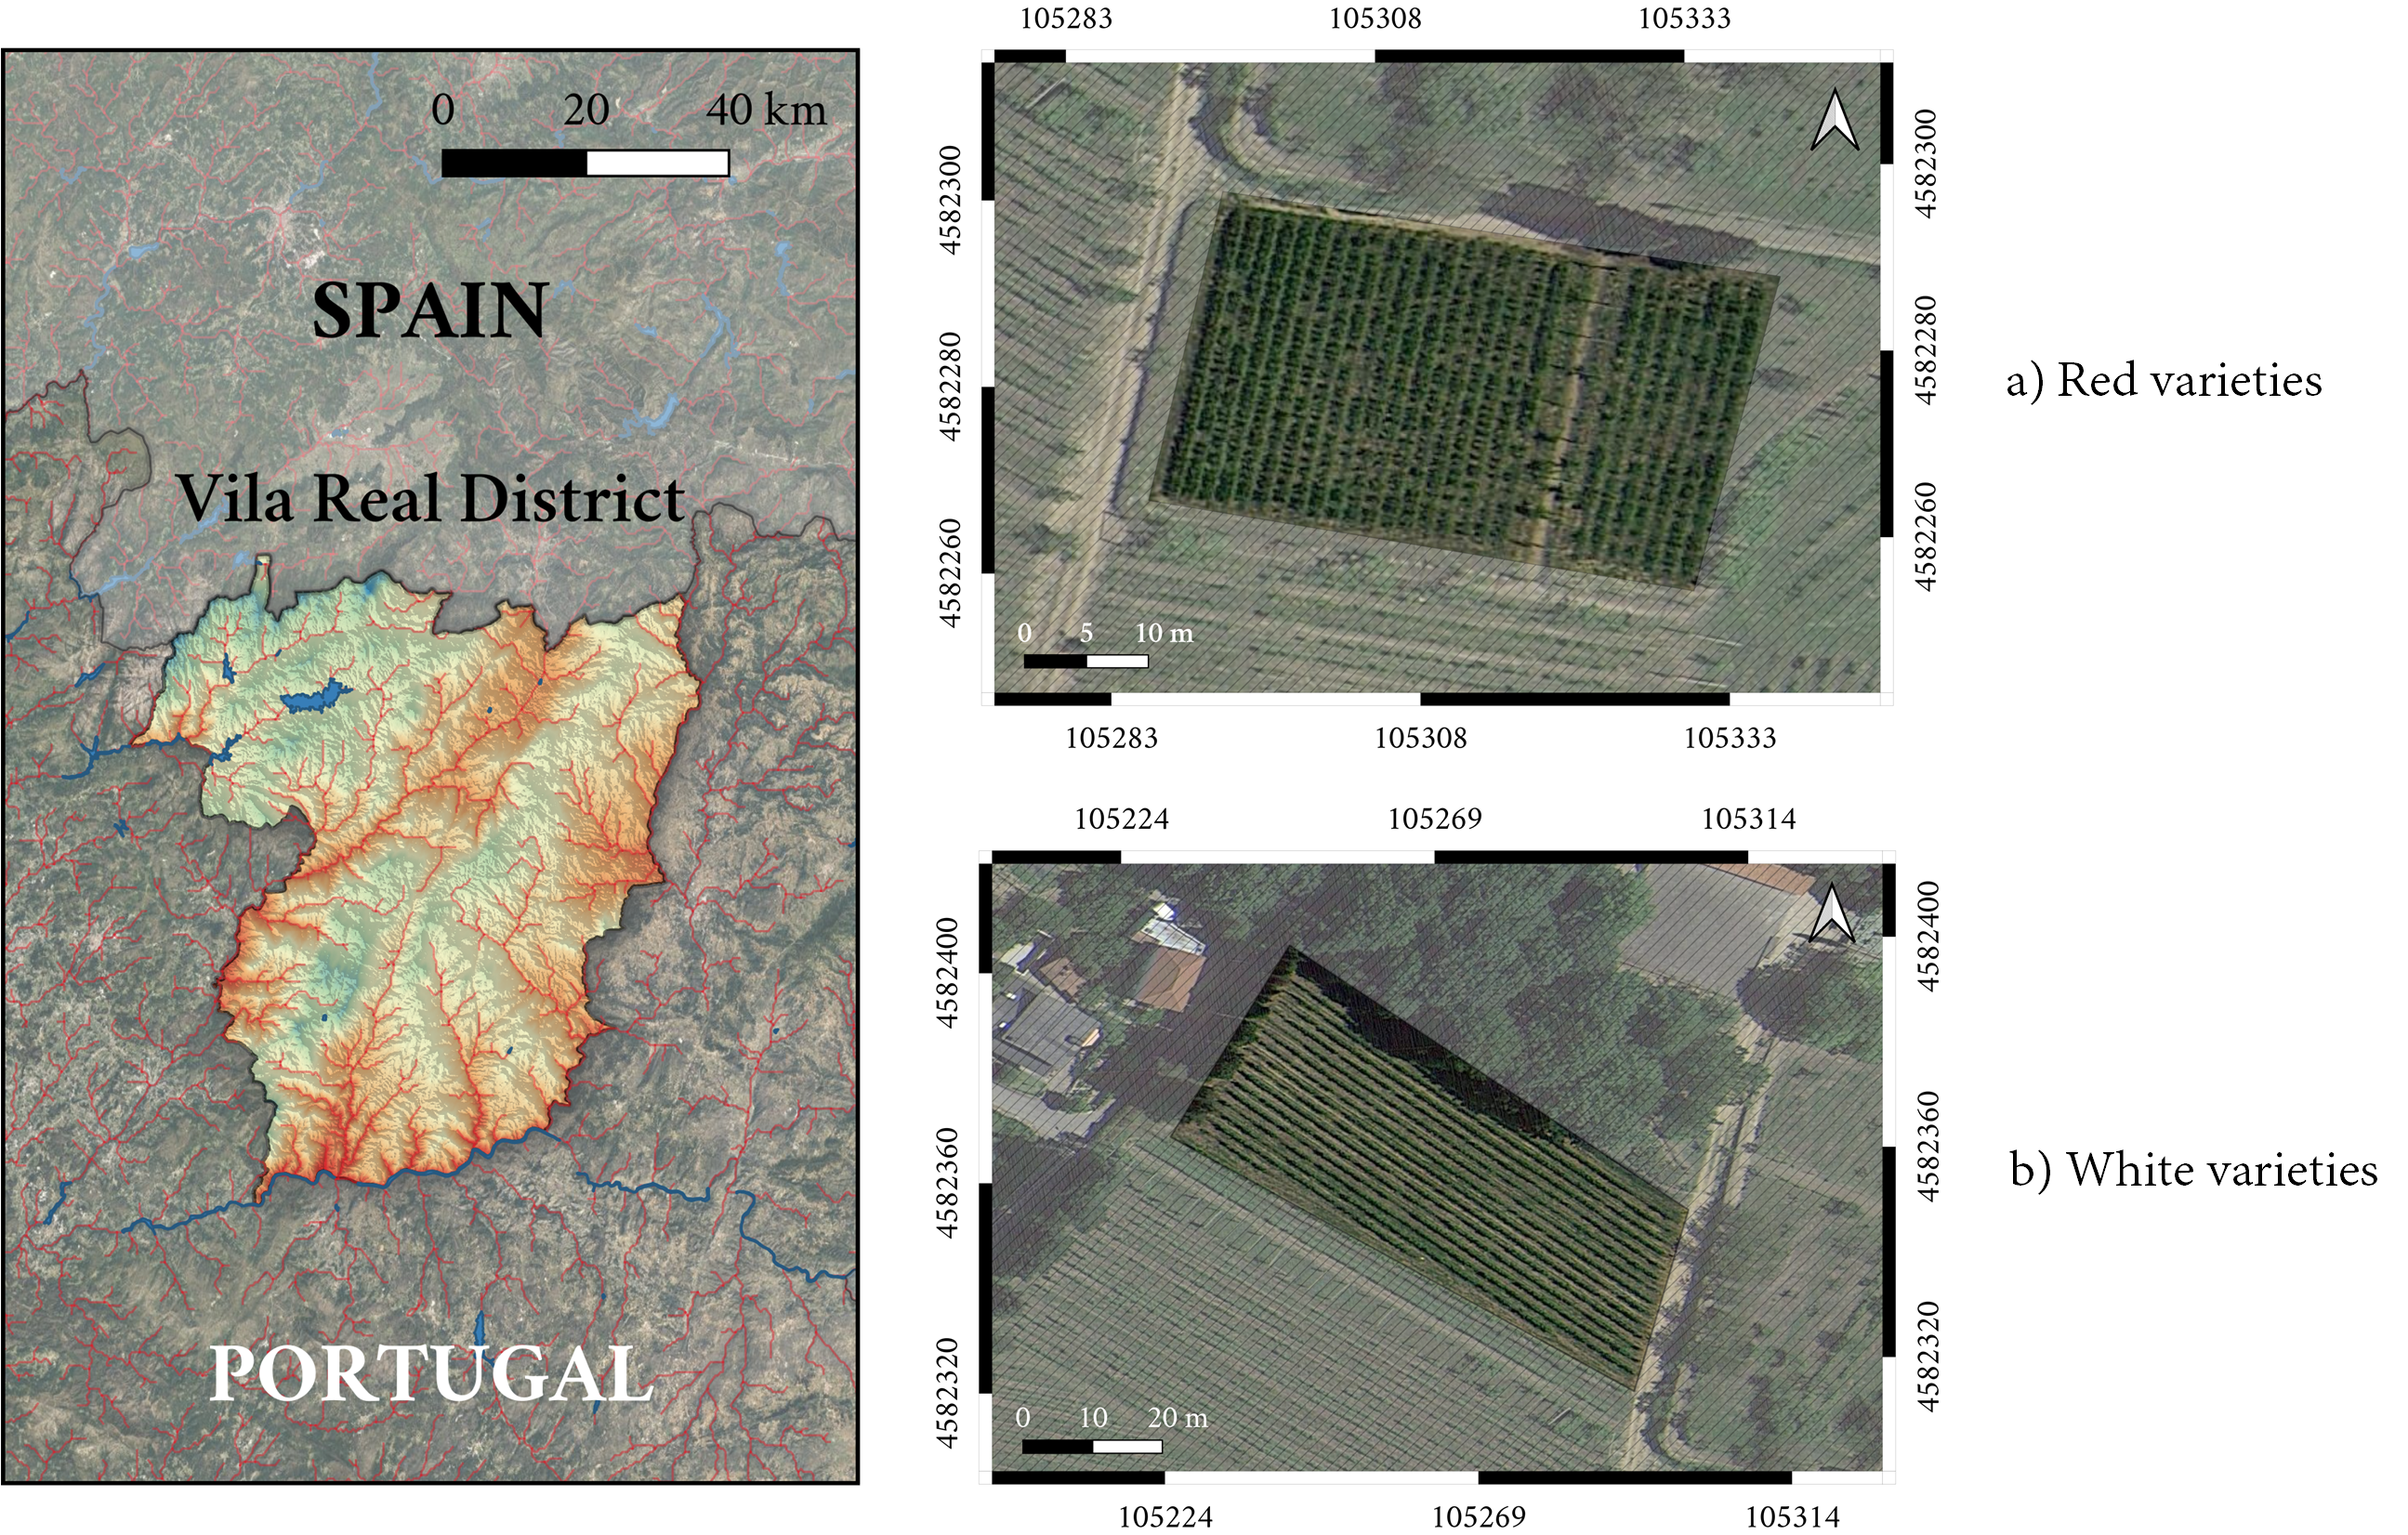
\includegraphics{figs/image_fusion/study_area.png}
    \caption{An overview of the study area. Coordinates are given in the Universal Transverse Mercator (\acrshort{utm}) coordinate system.}
    \label{fig:image_fusion_study_area}
\end{figure*}

The measurements were performed on a computer with Intel Core i7.6700 3.4GHz, 16GB RAM, NVIDIA GTX 1070 with 8GB RAM and Windows 10 operative system (\acrshort{os}). The implementation of the \acrshort{ecc} algorithm was provided by the image processing library Open Source Computer Vision Library (\acrshort{opencv}) in a C++ application. The accuracy of the matching process was estimated using the normalized \acrshort{cc}, defined as shown in Equation \ref{ec:correlation_coefficient}. The \acrshort{cc} metric obtains a coefficient $\rho \in [0, 1]$ that measures the similarity between two images $I$ and $T$, coined as source and template. It estimates the intensity difference between two images to shed light on the matching accuracy, although it is not a perfect measurement of how similar are two images. Finally, the images to be compared were randomly selected from the four datasets.
\begin{equation}
    \label{ec:correlation_coefficient}
    \textit{CC} = \frac{\sum_{x',y'} T(x',y') * I(x + x', y + y')}{\sqrt{\sum_{x',y'}T(x',y')^{2} * \sum_{x',y'}I(x + x',y + y')^{2}}}
\end{equation}

The response time and registration accuracy were checked against several configurations that include the following parameters: 
\begin{itemize}
    \item \textbf{Precision to converge}. The closer it gets to zero, the harder is for the algorithm to converge.
    \item \textbf{Number of iterations}. A larger number of iterations helps to give some room for the algorithm to converge. 
    \item \textbf{Image size}. A smaller dimensionality helps to decrease the response time and achieve faster convergence, and it does not necessarily lead to worse matching results. 
\end{itemize}

\subsection{Multispectral registration}

Four experiments were carried out to check the accuracy of the registration methodology using the four multispectral bands. The starting \acrshort{cc} is presented in Table \ref{table:multispectral_base_correlation} to highlight the improvement of the four image-matching experiments against the initial scenario. The dimensionality of multispectral images is low and therefore did not require to be downscaled. The first experiment used parameters that may be near the optimal configuration, at the expense of a higher response time. Table \ref{table:multispectral_rgb_correlation} shows that worse results were obtained for images showing human-made objects whose intensity difference was notably more significant amongst several spectral bands. Still, these were well aligned by visual inspection. The second test shows how the response time decreased at the expense of obtaining a lower \acrshort{cc}. The third experiment used an in-between configuration with respect to the previous: it achieved a high \acrshort{cc} but also decreased the latency. Finally, the fourth experiment downscaled the image size by $1/3$, obtaining a higher \acrshort{cc} with a lower response time. However, the latter returns worse results by visual inspection.

\textit{The configuration of the four experiments was the following. Test 1: $n \gets 30, p \gets 1^{-10}$, test 2: $n \gets 15, p \gets 1^{-2}$, test 3: $n \gets 15, p \gets 1^{-10}$ and test 4: $n \gets 150, p \gets 1^{-60}$}.

\renewcommand{\arraystretch}{1.2}
\begin{table}
    \caption{Normalized \acrshort{cc} between original multispectral images. }
    \label{table:multispectral_base_correlation}
    \begin{tabular}{ll|c@{\hskip 0.2in}c@{\hskip 0.2in}c}
        \toprule
        & & GRE-RED & GRE-\acrshort{nir} & GRE-\acrshort{reg} \\
        \cmidrule{1-5}
        Dataset & Viewpoint & $\rho$ & $\rho$ & $\rho$ \\
        \cmidrule{1-5}
        \multirow{3}{*}{1} & 1 & 0.8954 & 0.8777 & 0.9306\\
        & 4 & 0.9777 & 0.9381 & 0.9618\\
        & 6 & 0.9756 & 0.9520 & 0.9727\\
        \cmidrule{1-5}
        \multirow{4}{*}{2} & 37 & 0.9286 & 0.9100 & 0.9371\\
        & 48 & 0.9265 & 0.8918 & 0.9316\\
        & 58 & 0.9146 & 0.8878 & 0.9242\\
        & 53 & 0.9777 & 0.9381 & 0.9618\\
        \cmidrule{1-5}
        \multirow{8}{*}{3} & 9 & 0.9669 & 0.9545 & 0.9714\\
        & 35 & 0.9578 & 0.9453 & 0.9739\\
        & 78 & 0.9707 & 0.9504 & 0.9672\\
        & 107 & 0.9602 & 0.9537 & 0.9686\\
        & 136 & 0.9755 & 0.9612 & 0.9692\\
        & 141 & 0.9732 & 0.9551 & 0.9744\\
        & 142 & 0.9728 & 0.9375 & 0.9656\\
        & 144 & 0.9731 & 0.9316 & 0.9622\\
        \cmidrule{1-5}
        \multicolumn{2}{r|}{\textbf{Average}} & \textbf{0.9564} & \textbf{0.9323} & \textbf{0.9581}\\
        \bottomrule
    \end{tabular}
    \normalsize
\end{table}
\renewcommand{\arraystretch}{1}

\renewcommand{\arraystretch}{1.2}
\begin{table*}
    \footnotesize
    \caption{Normalized correlation coefficient and response time on the matching of a random subset of multispectral images over four different tests.}
    \label{table:multispectral_correlation_registration}
    \begin{tabular}{ll|cccr|cccr}
        \toprule
        \multicolumn{2}{c}{} & \multicolumn{4}{c}{Test 1} & \multicolumn{4}{c}{Test 2}\\
        \cmidrule{1-10}
        & & GRE-RED & GRE-\acrshort{nir} & GRE-\acrshort{reg} & & GRE-RED & GRE-\acrshort{nir} & GRE-\acrshort{reg}\\
        Dat. & Viewpoint & $\rho$ & $\rho$ & $\rho$ & \#time (\si{\second}) & $\rho$ & $\rho$ & $\rho$ & \#time (\si{\second}) \\
        \cmidrule{1-10}
        \multirow{3}{*}{1} & 1 & 0.9545 & 0.9186 & 0.9403 & 3.627 & 0.9545 & 0.9181 & 0.9395 & 1.128\\
        & 4 & 0.9888 & 0.9473 & 0.9681 & 3.576 & 0.9814 & 0.9473 & 0.9681 & 950\\
        & 6 & 0.9861 & 0.9591 & 0.9772 & 3.622 & 0.9817 & 0.9591 & 0.9767 & 1.079\\
        \cmidrule{1-10}
        \multirow{4}{*}{2} & 48 & 0.9654 & 0.9107 & 0.9368 & 3.580 & 0.9654 & 0.9107 & 0.9368 & 1.282\\
        & 58 & 0.9546 & 0.9088 & 0.9321 & 3.607 & 0.9547 & 0.9088 & 0.9321 & 1.224\\
        & 53 & 0.9888 & 0.9473 & 0.9681 & 3.573 & 0.9814 & 0.9473 & 0.9681 & 955\\
        & 37 & 0.9628 & 0.9265 & 0.9461 & 3.569 & 0.9463 & 0.9265 & 0.9460 & 1.100\\
        \cmidrule{1-10}
        \multirow{8}{*}{3} & 35 & 0.9973 & 0.9654 & 0.9785 & 3.543 & 0.9973 & 0.9645 & 0.9766 & 1.090\\
        & 107 & 0.9973 & 0.9621 & 0.9776 & 3.558 & 0.9973 & 0.9621 & 0.9776 & 1.356\\
        & 136 & 0.9973 & 0.9677 & 0.9767 & 3.577 & 0.9781 & 0.9623 & 0.9760 & 581\\
        & 78 & 0.9957 & 0.9640 & 0.9731 & 3.575 & 0.9956 & 0.9615 & 0.9696 & 1.353\\
        & 142 & 0.9962 & 0.9632 & 0.9749 & 3.567 & 0.9772 & 0.9632 & 0.9748 & 989\\
        & 144 & 0.9964 & 0.9580 & 0.9715 & 3.586 & 0.9781 & 0.9580 & 0.9715 & 994\\
        & 9 & 0.9967 & 0.9713 & 0.9810 & 3.585 & 0.9967 & 0.9713 & 0.9810 & 1.471\\
        & 141 & 9966 & 0.9746 & 0.9791 & 3.518 & 0.9967 & 0.9713 & 0.9810 & 1.110\\
        \cmidrule{1-10}
        \multicolumn{2}{r|}{\textbf{Average}} & \textbf{0.9849} & \textbf{0.9496} & \textbf{0.9654} & \textbf{3.5775} & \textbf{0.9788} & \textbf{0.9488} & \textbf{0.965} & \textbf{1.1108}\\
        \cmidrule{1-10}
        \multicolumn{2}{r|}{\textbf{Starting results}} & 0.9564 & 0.9323 & 0.9581 & & 0.9564 & 0.9323 & 0.9581 & \\
        \bottomrule
    \end{tabular}
    \normalsize
\end{table*}
\renewcommand{\arraystretch}{1}

\renewcommand{\arraystretch}{1.2}
\begin{table*}
    \footnotesize
    \caption{Continuation of Table \ref{table:multispectral_correlation_registration}.}
    \begin{tabular}{ll|cccr|cccr}
        \toprule
        \multicolumn{2}{c}{} & \multicolumn{4}{c}{Test 3} & \multicolumn{4}{c}{Test 4}\\
        \cmidrule{1-10}
        & & GRE-RED & GRE-\acrshort{nir} & GRE-\acrshort{reg} & & GRE-RED & GRE-\acrshort{nir} & GRE-\acrshort{reg}\\
        Dat. & Viewpoint & $\rho$ & $\rho$ & $\rho$ & \#time (\si{\second}) & $\rho$ & $\rho$ & $\rho$ & \#time (\si{\second}) \\
        \cmidrule{1-10}
        \multirow{3}{*}{1} & 1 & 0.9545 & 0.9186 & 0.9403 & 1.933 & 0.9540 & 0.9181 & 0.9394 & 1.797\\
        & 4 & 0.9866 & 0.9474 & 0.9682 & 1.900 & 0.9883 & 0.9473 & 0.9665 & 1.780\\
        & 6 & 0.9838 & 0.9592 & 0.9772 & 1.927 & 0.9849 & 0.9610 & 0.9767 & 1.818\\
        \cmidrule{1-10}
        \multirow{4}{*}{2} & 48 & 0.9654 & 0.9107 & 0.9367 & 1.884 & 0.9651 & 0.9113 & 0.9368 & 1.746\\
        & 58 & 0.9546 & 0.9088 & 0.9321 & 1.994 & 0.9651 & 0.9113 & 0.9368 & 1.774\\
        & 53 & 0.9866 & 0.9474 & 0.9682 & 1.921 & 0.9883 & 0.9473 & 0.9665 & 1.760\\
        & 37 & 0.9628 & 0.9265 & 0.9461 & 1.895 & 0.9618 & 0.9266 & 0.9455 & 1.774\\
        \cmidrule{1-10}
        \multirow{8}{*}{3} & 35 & 0.9973 & 0.9654 & 0.9785 & 1.905 & 0.9972 & 0.9659 & 0.9778 & 1.805\\
        & 107 & 0.9973 & 0.9621 & 0.9776 & 1.920 & 0.9970 & 0.9618 & 0.9762 & 1.788\\
        & 136 & 0.9966 & 0.9645 & 0.9766 & 1.900 & 0.9969 & 0.9671 & 0.9752 & 1.761\\
        & 78 & 0.9957 & 0.9640 & 0.9731 & 1.903 & 0.9948 & 0.9633 & 0.9714 & 1.798\\
        & 142 & 0.9941 & 0.9632 & 0.9749 & 1.909 & 0.9961 & 0.9632 & 0.9740 & 1.773\\
        & 144 & 0.9909 & 0.9580 & 0.9715 & 1.898 & 0.9963 & 0.9580 & 0.9702 & 1.774\\
        & 9 & 0.9967 & 0.9713 & 0.9810 & 1.911 & 0.9964 & 0.9713 & 0.9806 & 1.789\\
        & 141 & 0.9966 & 0.9746 & 0.9791 & 1.873 & 0.9965 & 0.9750 & 0.9786 & 1.789\\
        \cmidrule{1-10}
        \multicolumn{2}{r|}{\textbf{Average}} & \textbf{0.9839} & \textbf{0.9493} & \textbf{0.9654} & \textbf{1.9048} & \textbf{0.9852} & \textbf{0.9499} & \textbf{0.9648} & \textbf{1.7817}\\
        \cmidrule{1-10}
        \multicolumn{2}{r|}{\textbf{Starting results}} & 0.9564 & 0.9323 & 0.9581 & & 0.9564 & 0.9323 & 0.9581 & \\
        \bottomrule
    \end{tabular}
    \normalsize
\end{table*}
\renewcommand{\arraystretch}{1}

\subsection{\acrshort{rgb} and multispectral image-matching}

Table \ref{table:multispectral_rgb_correlation} shows the results of three different experiments. Note that changes in the observed intensity are even more significant in \acrshort{rgb} and multispectral imagery, thus hardening the image-matching and increasing the response time. The second test obtains the lowest latency, while the first achieves the same result with increased response time. This scenario proves the convergence of the \acrshort{ecc} algorithm. The safest approach is to select a large number of iterations that ensures convergence, whereas a real-time application may be better suited for a lower number of iterations at the expense of not converging. Both tests used images with a size equal to the multispectral dimensionality split by two. Such size enables smoothing the image and improving the image-matching, despite a small blur still being required. The third test used the starting multispectral size and \acrshort{rgb} images were downscaled to fit them. It returned worse results than previous tests since the number of iterations and precision were reduced to avoid high latency. 

\textit{The configurations of the three experiments are the following. Test 1: $d \gets \textit{d}_{\textit{mult.}} / 2, n \gets 400, p \gets 1\textsuperscript{-60}$, test 2: $d \gets \textit{d}_{\textit{mult.}} / 2, n \gets 150, p \gets 1\textsuperscript{-30}$ and test 3: $d \gets \textit{d}_{\textit{mult.}}, n \gets 100, p \gets 1\textsuperscript{-20}$}.

\renewcommand{\arraystretch}{1.2}
\begin{table}
    \footnotesize
    \caption{Normalized \acrshort{cc} and response time on the matching of a random subset of multispectral and \acrshort{rgb} images from the fourth dataset.}
    \label{table:multispectral_rgb_correlation}
    \begin{tabular}{l|cc|cc|cc}
        \toprule
        \multicolumn{1}{c}{} & \multicolumn{2}{c}{Test 1} & \multicolumn{2}{c}{Test 2} & \multicolumn{2}{c}{Test 3}\\
        \cmidrule{1-7}
        Viewpoints & $\rho$ & \#time (\si{\second}) & $\rho$ & \#time (\si{\second}) & $\rho$ & \#time (\si{\second})\\
        \cmidrule{1-7}
        1, 916 & 0.9683 & 8.090 & 0.9683 & 2.810 & 0.9569 & 7.405\\
        148, 918 & 0.9664 & 7.882 & 0.9664 & 2.839 & 0.9408 & 7.022\\
        142, 904 & 0.9711 & 7.506 & 0.9711 & 2.757 & 0.9453 & 7.058\\ 
        137, 892 & 0.9761 & 7.221 & 0.9761 & 2.718 & 0.9747 & 7.448\\
        144, 906 & 0.9690 & 7.266 & 0.9690 & 2.724 & 0.9680 & 7.087\\
        \cmidrule{1-7}
        \multicolumn{1}{r|}{\textbf{Average}} & \textbf{0.970} & \textbf{7593} & \textbf{0.9701} & \textbf{2.769} & \textbf{0.9571} & \textbf{7.204}\\
        \bottomrule
    \end{tabular}
    \normalsize
\end{table}
\renewcommand{\arraystretch}{1}

\subsection{Thermal and \acrshort{rgb} image-matching}

Three experiments were performed with the same parameters as before (Table \ref{table:thermal_rgb_correlation}). In comparison with previous tests, reducing the image dimensionality did not have a great impact on the results since edges are smoothed out in \acrshort{ir} images. \acrshort{cc} values were also lower than in previous tests since the registration results have areas with null values, as shown in Figure \ref{fig:thermal_comparative}. Therefore, the first and third tests show the aftermath of data being downscaled to the dimensionality of thermal images. Both reached the best \acrshort{cc}, whereas the third experiment returned the same results as the first, although with faster convergence and lower response time. The second experiment utilized the original thermographic size and obtained almost the same \acrshort{cc} at the cost of a slightly higher response time. In contrast with multispectral tests, the first and third experiments used images with smaller dimensionality but the results were not as inaccurate by visual inspection. From here, it could be concluded that thermal imagery can be matched with \acrshort{rgb} data by downscaling the dimensionality of both to fasten the convergence. 

\textit{The three experiments that were carried out used the following configuration. Test 1: $d \gets \textit{d}_{\textit{thermal}} / 2, n \gets 300, p \gets 1\textsuperscript{-60}$, test 2: $d \gets \textit{d}_{\textit{thermal}}, n \gets 100, p \gets 1\textsuperscript{-20}$ and test 3: $d \gets \textit{d}_{\textit{thermal}} / 2, n \gets 60, p \gets 1\textsuperscript{-20}$}.

\renewcommand{\arraystretch}{1.15}
\begin{table*}[ht]
    \small
    \caption{Normalized \acrshort{rgb} and response time on the matching of a random subset of \acrshort{rgb} and thermal images over three different tests.}
    \label{table:thermal_rgb_correlation}
    \begin{tabular}{ll|cr|cr|cr}
        \toprule
        \multicolumn{2}{c}{} & \multicolumn{2}{c}{Test 1} & \multicolumn{2}{c}{Test 2} & \multicolumn{2}{c}{Test 3}\\
        \toprule
        Dataset & Viewpoint & $\rho$ & \#time (\si{\second}) & $\rho$ & \#time (\si{\second}) & $\rho$ & \#time (\si{\second})\\
        \cmidrule{1-8}
        \multirow{8}{*}{3} & 394 & 0.9756 & 2.779 & 0.9771 & 3.204 & 0.9756 & 1.419\\
        & 626 & 0.9728 & 2.834 & 0.9745 & 3.320 & 0.9728 & 1.389\\
        & 726 & 0.9728 & 2.951 & 0.9741 & 3.211 & 0.9728 & 1.411\\ 
        & 928 & 0.9756 & 2.761 & 0.9770 & 3.341 & 0.9756 & 1.401\\
        & 467 & 0.9416 & 2.731 & 0.9385 & 3.134 & 0.9417 & 1.381\\
        & 643 & 0.9511 & 2.789 & 0.9494 & 3.137 & 0.9511 & 1.404\\ 
        & 963 & 0.9444 & 2.881 & 0.9425 & 3.177 & 0.9444 & 1.403\\
        & 475 & 0.9396 & 2.946 & 0.9358 & 3.257 & 0.9396 & 1.390\\
        \cmidrule{1-8}
        \multirow{4}{*}{4} & 922 & 0.9674 & 2.791 & 0.9690 & 3200 & 0.9674 & 1.396\\
        & 554 & 0.9786 & 2.790 & 0.9803 & 3.267 & 0.9786 & 1.402\\
        & 405 & 0.9266 & 2.716 & 0.9265 & 3.187 & 0.9266 & 1.400\\
        & 607 & 0.9511 & 2.794 & 0.9502 & 3.236 & 0.9511 & 1.382\\
        \cmidrule{1-8}
        \multicolumn{2}{r|}{\textbf{Average}} & \textbf{0.958} & \textbf{2.8135} & \textbf{0.9579} & \textbf{3.222} & \textbf{0.9581} & \textbf{1.398}\\
        \bottomrule
    \end{tabular}
    \normalsize
\end{table*}
\renewcommand{\arraystretch}{1}

\section{Conclusions}

In this chapter, a framework for matching images collected from multiple remotely sensed datasets was proposed. These datasets were acquired from \acrshort{uas} to help in the generation of multi-layer model with high \acrshort{lod}. To enable the registration of multiple images, the Enhanced Correlation Coefficient, \acrshort{ecc}, was proven to be very convenient for images that have notable colourimetric differences, as a result of being sensitive to distinct spectral wavelengths. Finally, a case study was explored over this multi-layer system. Individual trees were identified and their shapes were reconstructed using the previously matched multispectral images, thus enabling applications such as multi-temporal tracking.

As a future work, this framework could be extended to images whose differences, especially regarding geometry, are larger. For instance, the changes in consecutive remotely sensed images are frequently smaller than collecting data with terrestrial surveys. Still, affine and homography transformations are required to approach the image-matching problem. From this work, an adaptive algorithm starting from a very reduced size, until reaching the original size, could be evaluated to work with images more sparsed in collection time. In this manner, reducing the size helps to find an approximate, yet imprecise, transformation with a lower response time, whereas using a higher dimensionality is better suited to estimate fine-grained transformations.

